%% Version 5.0, 2 January 2020
%
%%%%%%%%%%%%%%%%%%%%%%%%%%%%%%%%%%%%%%%%%%%%%%%%%%%%%%%%%%%%%%%%%%%%%%
% TemplateV5.tex --  LaTeX-based template for submissions to the 
% American Meteorological Society
%
%%%%%%%%%%%%%%%%%%%%%%%%%%%%%%%%%%%%%%%%%%%%%%%%%%%%%%%%%%%%%%%%%%%%%
% PREAMBLE
%%%%%%%%%%%%%%%%%%%%%%%%%%%%%%%%%%%%%%%%%%%%%%%%%%%%%%%%%%%%%%%%%%%%%

%% Start with one of the following:
% DOUBLE-SPACED VERSION FOR SUBMISSION TO THE AMS
\documentclass{ametsocV5}

% TWO-COLUMN JOURNAL PAGE LAYOUT---FOR AUTHOR USE ONLY
% \documentclass[twocol]{ametsocV5}


% Enter packages here. If too many math alphabets are used,
% remove unnecessary packages or define hmmax and bmmax as necessary.

%\newcommand{\hmmax}{0}
%\newcommand{\bmmax}{0}
\usepackage{amsmath,amsfonts,amssymb,bm}
\usepackage{mathptmx}%{times}
\usepackage{newtxtext}
%\usepackage{newtxmath}


%%%%%%%%%%%%%%%%%%%%%%%%%%%%%%%%

%%% To be entered by author:

%% May use \\ to break lines in title:

\title{Snowfall model validation using surface observations and an optimal estimation snowfall retrieval}

%%% Enter authors' names, as you see in this example:
%%% Use \correspondingauthor{} and \thanks{Current Affiliation:...}
%%% immediately following the appropriate author.
%%%
%%% Note that the \correspondingauthor{} command is NECESSARY.
%%% The \thanks{} commands are OPTIONAL.

    %\authors{Author One\correspondingauthor{Author name, email address}
% and Author Two\thanks{Current affiliation: American Meteorological Society, 
    % Boston, Massachusetts.}}

\authors{Franziska Hellmuth\correspondingauthor{Franziska Hellmuth, franziska.hellmuth@geo.uio.no}}

%% Follow this form:
    % \affiliation{American Meteorological Society, 
    % Boston, Massachusetts}

\affiliation{Department of Geosciences, University of Oslo, Oslo, Norway}

%% If appropriate, add additional authors, different affiliations:
    %\extraauthor{Extra Author}
    %\extraaffil{Affiliation, City, State/Province, Country}

\extraauthor{Bjørg Jenny Kokkvoll Engdahl}
\extraaffil{Norwegian Meteorological Institute, Oslo, Norway, and Department of Geosciences, University of Oslo, Oslo, Norway}

%% May repeat for a additional authors/affiliations:
\extraauthor{Trude Storelvmo}
\extraaffil{Department of Geosciences, University of Oslo, Oslo, Norway}

\extraauthor{Robert O. David}
\extraaffil{Department of Geosciences, University of Oslo, Oslo, Norway}

\extraauthor{Steven J. Cooper}
\extraaffil{University of Utah, Salt Lake City, Utah}

%\extraauthor{}
%\extraaffil{}

%%%%%%%%%%%%%%%%%%%%%%%%%%%%%%%%%%%%%%%%%%%%%%%%%%%%%%%%%%%%%%%%%%%%%
% ABSTRACT
%
% Enter your abstract here
% Abstracts should not exceed 250 words in length!
%
 

\abstract{
    In the wintertime, orographic precipitation falls as snow in the mid to high latitudes where it causes avalanches, affects local infrastructure, or leads to flooding during the spring thaw. Predicting snowfall amounts in mountainous regions is a challenge due to complex interactions between the local topography and dynamics. We present a technique to validate operational forecasts in complex terrain using a combination of remote sensing and in situ snowfall measurements.\\
    A Micro Rain Radar, a Precipitation Imaging Package, and a Multi-Angle Snowflake Camera provide microphysical information used in an optimal estimation retrieval (OESR). The validation of snowfall forecasts uses the winter 2016-2017 season when these instruments were deployed at the Haukeliseter test site in Norway.\\ 
    Retrieved surface snowfall is validated against measurements conducted with a double-fence automated reference gauge. The comparison shows that the OESR produces +10.9\,\% surface snowfall. The predicted surface snowfall from the operational forecast model MetCoOp ensemble prediction system (MEPS) and two additional simulations with microphysical adjustments (CTRL and ICE-T) show an overestimation at the surface of +41.0\,\%, +43.8\,\%, and +59.2\,\% for MEPS, the CTRL, and ICE-T, respectively. At the same time, the CTRL and ICE-T simulations underestimate the mean snow water path by -1071.4\,\%, and -523.7\,\%, respectively. Thus, simulations overestimate the amount of accumulated surface precipitation while underestimating the amount of snowfall present in the vertical. These results highlight the need for further studies to better constrain the interplay between the evolution of snow in the vertical and snowfall at the surface in numerical weather prediction models.
}

\begin{document}

%% Necessary!
\maketitle

%%%%%%%%%%%%%%%%%%%%%%%%%%%%%%%%%%%%%%%%%%%%%%%%%%%%%%%%%%%%%%%%%%%%%
% SIGNIFICANCE STATEMENT/CAPSULE SUMMARY
%%%%%%%%%%%%%%%%%%%%%%%%%%%%%%%%%%%%%%%%%%%%%%%%%%%%%%%%%%%%%%%%%%%%%
%
% If you are including an optional significance statement for a journal article or a required capsule summary for BAMS 
% (see www.ametsoc.org/ams/index.cfm/publications/authors/journal-and-bams-authors/formatting-and-manuscript-components for details), 
% please apply the necessary command as shown below:
%
% \statement
% Significance statement here.
%
% \capsule
% Capsule summary here.


%%%%%%%%%%%%%%%%%%%%%%%%%%%%%%%%%%%%%%%%%%%%%%%%%%%%%%%%%%%%%%%%%%%%%
% MAIN BODY OF PAPER
%%%%%%%%%%%%%%%%%%%%%%%%%%%%%%%%%%%%%%%%%%%%%%%%%%%%%%%%%%%%%%%%%%%%%
%

%% In all cases, if there is only one entry of this type within
%% the higher level heading, use the star form: 
%%
% \section{Section title}
% \subsection*{subsection}
% text...
% \section{Section title}

%vs

% \section{Section title}
% \subsection{subsection one}
% text...
% \subsection{subsection two}
% \section{Section title}

%%%
% \section{First primary heading}

% \subsection{First secondary heading}

% \subsubsection{First tertiary heading}

% \paragraph{First quaternary heading}


%%% Introduction %%%%%%%%%%%%%%%%%%%%%%%%%%%%%%%%%%%%%%%%%%%%%%%%%%%
\section{Introduction}
    Orographic precipitation is important for the hydrological cycle and climate, as more than one-sixth of the world’s population receives water from glaciers and seasonal snowpacks \citep{barnett_potential_2005}. As such, the topic has been a long-standing focus for both weather and climate research communities \citep{stoelinga_improvement_2003,schar_orographic_2005,ranzi_hydrological_2007}.
%    
    Forecasting precipitation quantitatively is challenging, especially in complex terrain, and the evaluation of forecast models is difficult in mountainous regions due to the sparse distribution of precipitation gauges \citep{barstad_evaluation_2005}. Furthermore, coarse numerical weather prediction (NWP) models have been shown to be less skillful in simulating orographic precipitation, especially over narrow topography \citep{gowan_validation_2018}. This difficulty is unfortunate, as forecasting of avalanches, glacier mass budgets, and flash floods depends on accurate models. 
    In order to validate snowfall predictions from models, accurate surface observations of precipitation are required. However, measuring precipitation, especially in the form of snow, is a well-known challenge. Airflow around the precipitation gauge can cause falling hydrometeors to bypass the gauge inlet, resulting in an underestimation of the true snowfall rate. This effect varies with wind speed, wind shielding, the hydrometeor type i.e. the crystal habit, and the fall velocity of the hydrometeor \citep{theriault_dependence_2012,wolff_measurements_2013,colli_improved_2015}. Winter precipitation measurements can show biases of more than 100\,\% relative to snow gauge observations where the exact bias values depend upon regional snowfall characteristics \citep{kochendorfer_analysis_2017}. At high wind speeds, precipitation loss can be severe. Additionally, snow can be lifted from the surface, enter the gauge, and artificially enhance the reported precipitation \citep{nitu_iom_2018}. A double fence automated reference (DFAR) gauge provides a more accurate estimate of snow accumulation compared to single fence gauges during high wind speeds \citep{wolff_derivation_2015,kochendorfer_analysis_2017}. Nevertheless, the DFAR still has an under-catch of 10\,\% at wind speeds below 9\,m\,s$^{-1}$ and 20\,\% under-catch at wind speeds between 9\,m\,s$^{-1}$ and 20\,m\,s$^{-1}$ \citep{nitu_iom_2018}. Such uncertainties must be considered when using gauge observations to evaluate both model snowfall forecasts and remote sensing algorithm estimates of snowfall \citep{wolff_derivation_2015}. 
    
    The quantitative estimates of snowfall from radar-based remote sensing techniques relies on deriving a snowfall rate (S) from a radar reflectivity (Z). Several studies have shown, however, that the estimated value of S depends critically upon the choice of microphysical assumptions required for the retrieval \citep{kulie_utilizing_2009,friedrich_quantifying_2020}. The selection of non-representative particle snowflake model or particle size distribution or fall speed for a given snowstorm Z profile can lead to significant errors in retrieved S. Thus, other studies have tried to incorporate scene-specific snowflake microphysical property information into the retrieval scheme to better match environmental conditions \citep{wood_microphysical_2015}. \citet{cooper_variational_2017}, for example, explored the use of in-situ observations of snowflake microphysical properties from the Multiple Angle Snow Camera (MASC) to improve radar-based estimates of snowfall at Barrow, Alaska. This study exploited an optimal estimation snowfall retrieval (OESR) approach that combined radar reflectivies, in-situ microphysical property estimates, and environmental information into a common retrieval framework to provide estimates of snowfall properties consistent with each. Retrieved snowfall values from the \citet{cooper_variational_2017} OESR technique differed by 18\,\% relative to nearby National Weather Service snow gauge measurements over multiple snow events, preliminarily suggesting that the approach worked well for winter conditions at Barrow.

    \citet{schirle_estimation_2019} applied the \citet{cooper_variational_2017} algorithm approach to the instrumentation and environmental conditions at the Haukeliseter Test Site (HTS). During winter season 2016-17, this site was additionally equipped with a Micro Rain Radar (MRR), Precipitation Imaging Package (PIP), and MASC as part of the National Science Foundation (NSF) High-Latitude Measurement of Snowfall (HiLaMS) campaign. Retrieved estimates of surface snowfall accumulation were calculated using different assumptions of snow PSDs, habit, and fall speed from the instruments and were evaluated against DFAR observations. Total retrieved seasonal snowfall values agreed to within +20\,\% of snow gauge measurements for the two predominant snowfall regimes observed during the campaign, again suggesting confidence in the OESR approach. 
    
    With the increasing expansion of computational power, NWP models with $\leq$4\,km resolution are now increasingly capable of a better representation of terrain, which is critical for accurately predicting precipitation in mountainous terrain \citep{colle_59_2000, colle_1314_2005, garvert_1314_2005, schwartz_reproducing_2014}. Nevertheless, the higher model resolution allows for a representation of small-scale phenomena such as convective dynamics \citep{gowan_validation_2018}, thus enabling more accurate simulations of the magnitude and location of maximum precipitation and local wind speed. This information is of significant importance for meteorological services, especially when warnings for severe weather events have to be communicated to the public.
    
    However, the implementation of high-resolution models is accompanied by various challenges, such as scale-dependence of physical parameterization schemes, accurate representation of topography, and assimilation of high-resolution data \citep{sun_convective-scale_2005}. Uncertainties on a convective scale can lead to rapid error growth \citep{lorenz_atmospheric_1969}, even in models with high resolution. Modeling centers, therefore, utilize high-resolution ensemble prediction to limit forecast uncertainty. For example, the Meteorological Cooperation on Operational Numerical Weather Prediction produces an Ensemble Prediction (MEPS) by perturbing the initial state for the deterministic run of the  AROME-MetCoOp model \citep{frogner_convection-permitting_2019}. 
    
    It was shown that early versions of MEPS produced too much cloud ice with its default ICE3 cloud microphysics scheme \citep{muller_arome-metcoop:_2017}. Therefore, changes were made to the microphysics scheme to improve the representation of fog, low-level clouds, and cirrus. More recently, \citet{engdahl_improving_2020} showed that even with the improvements, the microphysics scheme depleted supercooled liquid water too quickly and hence, produced a surplus of snow and graupel. For this reason, \citet{engdahl_improving_2020} introduced a series of changes to the ICE3 scheme based on the parameterization development by \citet{thompson_explicit_2004,thompson_explicit_2008}. The modified microphysics include an updated ice nucleation parameterization, a new parametrization for the collection of liquid water drops by solid hydrometeors (riming/accretion), and changes to the PSD of the rain class \citep{engdahl_improving_2020}. Idealized 1D experiments showed that the modified scheme prolonged the existence and produced higher amounts of supercooled liquid water \citep{engdahl_improving_2020}.

    Observations of vertical reflectivity provide information about the initiation, growth, and vertical distribution of precipitation in clouds. In particular, the retrieved vertical profiles of reflectivity can be used to validate cloud microphysical parameterizations. In addition to contributing to better representation of surface precipitation, improved microphysical parameterizations can influence the distribution of latent heat release, and hence the generation of potential vorticity which in turn controls if a storm strengthens or weakens \citep{joos_influence_2012}. Sensitivity tests varying the microphysical scheme of the Consortium for Smallscale Modelling model showed that storm development depended on the correct vertical placement of the precipitation inside a modeled storm \citep{joos_influence_2012}. Therefore, accurate vertical precipitation observations are required to evaluate model vertical precipitation patterns. Here, we present a novel technique using vertical observations of snow reflectivity to validate a regional forecast model both at the ground and in the atmospheric column above.

    In this study, we evaluate the performance of snowfall simulations at the surface and in the vertical during winter 2016-2017. We use snow observations from a double-fence automated reference (DFAR), radar-based snowfall retrieval \citep{cooper_variational_2017,schirle_estimation_2019}, and high-resolution forecast data from the operational forecast model MEPS at the Haukeliseter site. This is a unique opportunity to investigate the radar snowfall retrieval best estimates by \citet{schirle_estimation_2019} and verify the operational MEPS as well as sensitivity simulations with adjusted cloud microphysics conducted described by \citet{engdahl_effects_2020}.
    
    We structure the remainder of this paper as follows: Section \ref{sec:methodology} describes the HTS, the \citet{schirle_estimation_2019} OESR to estimate the vertical profile of snowfall, and the two distinct snowfall regimes observed during HiLaMS. Additionally, we present the operational ensemble forecast model MEPS, and two additional model runs by \citet{engdahl_effects_2020}. In \citet{engdahl_effects_2020} and in this study, CTRL includes a few modifications, but is assumed to be similar to the MEPS control run, while ICE-T is the model simulations with the implementation of an adjusted microphysical scheme. We also describe the  validation procedure of the forecast model simulations MEPS, CTRL, and ICE-T. Section \ref{sec:res} describes the snowfall regimes and the meteorological conditions, followed by the validation of the OESR retrieved solid surface accumulated precipitation with the DFAR measurements for the two snowfall wind regimes. Next, we discuss the seasonal bias in the accumulated solid surface precipitation by snowfall wind regimes in the forecast models (MEPS, CTRL, and ICE-T). The simulated vertical snowfall distribution of CTRL and ICE-T is compared to the snow water content profiles derived from the OESR. Finally, the conclusions are presented in Section \ref{sec:conclusion}.


%%%%%%%%%%%%%%%%%%%%%%%%%%%%%%%%%%%%%%%%%%%%%%%%%%%%%%%%%%%%%%%%%%%%%

%%% Methodology %%%%%%%%%%%%%%%%%%%%%%%%%%%%%%%%%%%%%%%%%%%%%%%%%%%%%
\section{Methodology}\label{sec:methodology}
    \subsection{Haukeliseter test site}
        The World Meteorological Organization (WMO) Haukeliseter test site (HTS), shown in Fig. \ref{fig:norway_map}, is situated on a mountain plateau at 991 m above sea level in Telemark County, Norway (59.81\textdegree N, 7.21\textdegree E). It has served as a WMO measurement site for snow accumulation since the winter of 2010-2011 \citep{wolff_new_2010} and is currently operated by the Norwegian Meteorological Institute (MET Norway). The HTS is shielded from passing storm systems to the west by mountain peaks that extend up to 500 m above the site. Meanwhile, winds from the east can reach the HTS almost unobstructed (see Fig \ref{fig:norway_map}).  
    
        The temperature, precipitation and wind are measured and recorded every minute at the HTS. Snowfall accounts for approximately 50\,\% of the annual precipitation at the site, and the snow depth typically reaches two to three meters \citep{wolff_derivation_2015}. Therefore, in this study, the temperature from the mast at 4.5\,m is used to represent the measurement of the 2-m air temperature. The wind speed and direction are measured by an anemometer mounted at a height of 10\,m, typically 8\,m above the snow surface. The dominant wind direction for snowfall is westerly and south-easterly with typical wind speeds below 20\,m\,s$^{-1}$ and 12\,m\,s$^{-1}$, respectively (see Fig. \ref{fig:windrose}). Precipitation at HTS is measured by a DFAR \citep{goodison_wmo_1998}, which consists of a precipitation-weighing gauge (Geonor T-200B3) encircled by a double fence, in order to reduce any impacts of high winds on the measurements. An overview of the instrumentation at HTS including the DFAR and the meteorological mast is shown in Fig. \ref{fig:instruments} a). 
    
        During the NSF HiLaMS field campaign, which took place at HTS during the 2016-2017 winter season, three additional instruments, a MASC, a PIP, and a MRR, were installed to study snowfall (see Fig. \ref{fig:instruments} b). The MASC (Fig. \ref{fig:instruments} b, left) consists of three cameras, three flashes, and two near-infrared sensors, pointing at a ring center. As a hydrometeor passes through the ring, it is detected by the near-infrared sensors, which trigger the flashes and cameras to obtain a three-dimensional image of the hydrometeor. Hydrometeor fall speed is determined from the time it takes to fall between the two vertically-arranged infrared sensors \citep{garrett_fall_2012}. The PIP (Fig. \ref{fig:instruments} b, middle) is a video disdrometer and consists of a halogen lamp and a video system sampling at 60\,Hz. The light source and lens have a distance of $\sim$3\,m that gives a field of view of 24\,mm by 32\,mm \citep{newman_presenting_2009}. The PIP and MASC together provided estimates of the snow crystal habit, PSD, and near-surface snow fall velocity, which were used to determine the OESR assumptions (see Sec. \ref{sec:methodology}\ref{sec:methodology:oesr}). Lastly, the MRR (Fig. \ref{fig:instruments}b, right) operates at 24\,GHz and was used to obtain particle reflectivity and Doppler velocity aloft, thus providing the vertical macrophysical structure of snow events. Profiles were retrieved with a temporal resolution of 1 minute and a vertical resolution of 100\,m between 300 and 3000\,m. 


    \subsection{Snowfall regime analysis}\label{sec:methodology:snowfall_reg}
        An analysis of 10-m wind (Fig. \ref{fig:windrose}) indicates that the majority of snowfall occurred in two distinct wind regimes at HTS. Furthermore, the MRR reflectivities indicate that the vertical structure of the precipitation also differed depending on the wind regime with the westerly events consisting of pulses of high reflectivites (\textgreater 25\,dbZ; see Fig. \ref{fig:MRR_refl}a). In contrast, the vertical reflectivity structure during the easterly wind regime was associated with light precipitation ($\leq$ 25\,dbZ; see Fig. \ref{fig:MRR_refl}b). Therefore, the snowfall events were separated by wind regime, namely a westerly (202.5\textdegree to 22.5\textdegree) and an easterly (22.5\textdegree to 202.5\textdegree) regime, similarly to \citet{schirle_estimation_2019}. This allows for the application of two different OESRs to retrieve the vertical structure of SWC and surface snowfall (see Sect. \ref{sec:methodology} \ref{sec:methodology:oesr}).
        
        The wind regime was assigned for each minutely observation when the surface temperature was less than 2\,$^{\circ}$C depending on the observed wind direction during that minute. However, to omit local topographic effects on the wind regime assignment, a given wind regime was only assigned if it lasted for more than 10 minutes. Thus wind shifts lasting less than 10 minutes, were assigned to the dominant encompassing wind direction. Once the wind regime was assigned to the minutely data, the respective OESR was used to calculate the surface accumulated snowfall and the vertical SWC. Due to instrument failures, only days with continuous hourly observations (24\,h) were considered in the analysis. Furthermore, to exclude measurement noise from the rest of the analysis, only minutes that occurred during days where more than 0.25\,mm\,d$^{-1}$ was observed by the both DFAR and OESR were used. 
        
        In order to compare the accumulated surface snowfall from the modeled hourly simulations with the DFAR surface accumulation, the DFAR measurements were summed over each hour and assigned to the instantaneous 10-m wind speed and direction at the end of the hour as measured by the anemometer at HTS. Similarly, the OESR surface accumulation was summed over each hour and assigned to the instantaneous wind speed and direction at the end of the hour, regardless of the OESR applied on a minutely basis during the hour. 
        We discuss the two distinct precipitation regimes with their specific meteorology, MRR reflectivities (Fig. \ref{fig:MRR_refl}) and associated snowfall in Section \ref{sec:res} \ref{sec:res:snowfall_regimes}.

    \subsection{Optimal Estimation Retrieval Algorithm}\label{sec:methodology:oesr}
        Estimates of the vertical profile of snow properties were derived from the OESR algorithm described in \citet{schirle_estimation_2019} for the instrumentation available at HTS. This retrieval scheme uses estimates of PSD, fall speed, and habit from the PIP and MASC to estimate surface snowfall rate and SWC from MRR reflectivity profiles. Use of the flexible optimal-estimation retrieval approach \citep{rodgers_inverse_2000} provides a means to combine radar reflectivities, in-situ observations, atmospheric temperature profiles, and a priori information into a common retrieval framework to provide an estimate of snowfall properties consistent with each. A priori information for the retrieval describes the probability distribution of snow PSD parameters as functions of temperature. The use of scene-dependent information allows for a range of possible retrieved snowfall values for a given MRR reflectivity value, which contrasts markedly with the use of traditional Z-S relationship techniques \citep{friedrich_quantifying_2020}.  
        
        Specifically, \citet{schirle_estimation_2019} determines the PSD slope parameter ($\lambda$) and number intercept ($N_0$) of an assumed exponential size distribution for each MRR range bin (Eq. \ref{eq:numberconc}).
        \begin{equation}
            n(r) = N_0 exp(-\lambda r)
            \label{eq:numberconc}
        \end{equation}
        These PSD parameters, in turn, can be used to calculate SWC in each layer through the use of snow particle size-mass dimensional relationships. SWC can then be transformed into precipitation rates through the use of fall speed observations from the MASC, PIP, or MRR. The selection of the particle model for the OESR is guided by the MASC images, which suggested predominantly rimed aggregates for HTS (see Fig. \ref{fig:snowflakes}). As such, a snow particle aggregate model \citep{wood_microphysical_2015} developed for the CloudSat mission was chosen due to its ability to produce the high reflectivity per unit mass relationship expected of aggregates entrained in high liquid water content aloft.  
        
        \citet{schirle_estimation_2019} found differences between total seasonal retrieved surface accumulations and HTS DFAR observations of +\,15\,\% and +\,9\% for the westerly and easterly snowfall regimes, respectively. However, the combination of measurements that maximized retrieval performance differed for these regimes due to variable sampling biases for disparate environmental conditions. For the high wind and snowfall westerly wind events, near-surface turbulence and blowing snow dictated the assumption of fall speed from the MRR and an a priori temperature PSD relationship. For the relatively low-wind easterly events, the use of in-situ observations of PSD and fall speed from the MASC worked well. In this work, these  assumptions are used to compare surface snowfall accumulations in the OESR with DFAR measurements for a slightly different classification scheme, described above,for snowfall events than those used in the \citet{schirle_estimation_2019}. Good agreement between retrieved and observed snowfall values at the surface, in turn, provide confidence in the retrieved SWC values aloft needed to evaluate the representation of snow water in MEPS, CTRL, and ICE-T.  

        
    \subsection{Operational Weather Forecast Model - MEPS}
        In this study, we use the results of the OESR together with DFAR measurements to validate the operational forecast model MEPS, and experiments with different microphysical adjustments. We make use of the archived MEPS surface forecasts, the control (CTRL) run, and a version of the CTRL with the modified microphysics scheme (ICE-T) from \citet{engdahl_effects_2020}.
        
        MEPS is the operational ensemble forecast model at MET Norway and runs in collaboration with the Swedish Meteorological and Hydrological Institute and the Finnish Meteorological Institute \citep{frogner_convection-permitting_2019}. MEPS is based on HARMONIE-AROME (version 40h1.1), a mesoscale non-hydrostatic, convection-permitting NWP model \citep{the_metcoop_team_metcoop_2017}. HARMONIE-AROME, in turn, is based on the model developed by Meteo-France, AROME \citep{seity_arome-france_2010,bengtsson_harmoniearome_2017}.
        
        HARMONIE-AROME uses the single-moment ICE3 bulk microphysics scheme \citep{bechtold_meso-nh_2009} to represent cloud microphysics. ICE3 simulates mass mixing ratios of cloud water and ice, rain, snow, and graupel \citep{cohard_comprehensive_2000, cohard_comprehensive_2000-1}. For all hydrometeors, the terminal speed velocity, $\upsilon$,  is related to the maximum ice particle diameter $D$ as shown in Eq. \ref{eq:fallvelo}.
        \begin{equation}
            \upsilon(D) = c D^d \left( \frac{\rho_{00}}{\rho_{dref}} \right)^{0.4}
            \label{eq:fallvelo}
        \end{equation}
        Each ice category has specific parameters depending on the habit and growth mode. Details about the constants $c$ and $d$ can be found in \citet{bechtold_meso-nh_2009}. $\rho_{00}$ represents the air density at sea level at the reference pressure level $p_{00}$ and $\rho_{dref}$ the air density at the particle height. 
        
        MEPS has a horizontal resolution of 2.5\,km with 65 hybrid levels in the vertical. Fig. \ref{fig:norway_map}a shows the MEPS model domain and simulated elevation with a domain center at 63\textdegree N, 15\textdegree E. MEPS consists of ten HARMONIE-AROME ensemble members. We use the ensemble output from the MEPS archive with initialization at 00\,UTC, with three-hourly cycling for data assimilation. The control run has initial and lateral boundary conditions from the European Centre for Medium-range Weather Forecasts (ECMWF) High Resolution forecast. The ensemble is created by giving members one through nine perturbed initial and lateral boundary conditions based on the Scaled Lagged Average Forecasting method \citep{koltzow_metcoop_2017}. In this study, the ensemble members are averaged (the ensemble mean) to derive the reported MEPS variables in the following figures. 
        
        A detailed description of the MEPS operational set-up can be found in \citet{frogner_convection-permitting_2019}. 
        
        In this study, we use the model simulations of \citet{engdahl_effects_2020}. They pointed out a coding error in the original scheme, which allowed heteorogeneous ice nucleation to occur only after ice was already present in the cloud, thus limiting initial freezing to homogeneous ice nucleation. This error was corrected in the CTRL run and therefore, the CTRL microphysics deviates from that of the archived MEPS simulations. 
        
        In a follow-up study, \citet{engdahl_effects_2020} ran 3D simulations with both the bug-fixed microphysics scheme (CTRL) and ICE-T, respectively for Dec 2016 - Feb 2017. An overview of the differences between the two microphysical schemes in CTRL and ICE-T is found in Table 1 in \citet{engdahl_improving_2020}. The \citet{engdahl_effects_2020} model setup is as follows: The domain has the same horizontal and vertical resolution as MEPS, but is placed further to the west \citep{frogner_harmonepsharmonie_2019} to provide additional spin-up time for weather systems from the west. The CTRL and ICE-T are initialized every day at 00\,UTC. The initialization uses the initial and lateral boundaries from the operational ECMWF-Integrated Forecast System, but with no surface or upper air data assimilation. Therefore clouds and precipitation are not available at the beginning of the simulation. \citet{engdahl_effects_2020} results showed that ICE-T led to a general increase in supercooled liquid water, a shift in hydrometeor distribution from graupel to snow, and a shift in the precipitation pattern with more precipitation spilling over to the lee side of mountain barriers.
        
         

    \subsection{Model validation}\label{sec:methodology:MEPS_vali}
        The winter season Dec 2016 - Feb 2017 simulations by \citet{engdahl_effects_2020} are used with each cycle starting at 00\,UTC. For the validation of the model, we use the closest grid point to HTS, which is located 0.9\,km from the site in MEPS and has a similar altitude of 1041\,m above sea level. Similar to \citet{engdahl_effects_2020}, we exclude the first 12 hours of each simulation and thereafter analyze the next 24\,h in order for model spin-up time of clouds and precipitation in MEPS, CTRL, and ICE-T. The DFAR and OESR data is allocated to the same times as the model simulations, hence a day of interest starts at 12\,UTC and ends the next day at 12\,UTC. Then the difference of the total accumulated precipitation within an hour is calculated for the observations and the model simulations. 
        Additionally, the instantaneous 2-m temperature of the observations and the model had to remain below 2\,$^{\circ}$C to ensure only snowfall is present due to the OESR setup, and resulting surface snowfall accumulation and SWC from the OESR. The separation into snowfall regimes is done by taking the instantaneous 10-m wind direction from MEPS, CTRL, and ICE-T. For analyzing the simulated surface solid accumulation and vertical precipitation by wind speed, the simulated wind speeds were corrected as \citet{frogner_convection-permitting_2019} found that MEPS often simulates higher wind speeds than observed. Indeed, during the development of MEPS the mean absolute error in 10-m wind speed continued to be more than 1.8\,m\,s$^{-1}$ over Norway. \citet{engdahl_effects_2020} verified CTRL and ICE-T with 177 WMO stations in Norway for the three winter months simulation and found the 10-m mean error in the wind speed to be around +0.7\,m\,s$^{-1}$. However, the complex terrain around the HTS and its representation in MEPS, CTRL, and ICE-T leads to the simulation of stronger wind bias (see Fig. \ref{fig:WS_correlation}). Therefore, an analysis of the simulated and observed wind speeds was done and a simulated bias of +2.92\,m\,s$^{-1}$, +2.44\,m\,s$^{-1}$, 2.55\,m\,s$^{-1}$ was found for MEPS, CTRL, and ICE-T, respectively (see Fig. \ref{fig:WS_correlation}). Therefore, the simulated wind speed was corrected in order to more accurately assign the solid surface accumulation and vertical precipitation to the corresponding observed wind speeds. 
        
        The MEPS archive does not provide the vertical parameters to calculate the SWC profile for all ensemble members. Hence, no vertical validation is carried out for MEPS simulations. Instead, we validate the instantaneous amount of snowfall in the vertical from the simulations CTRL (which we assume is close to the deterministic forecast in MEPS) and ICE-T to the OESR vertical profiles of SWC.
        
        In CTRL and ICE-T the SWCs were derived by summing the mass mixing ratios of cloud ice, snow, and graupel and then converting to g\,m$^{-3}$ (Eq. \ref{eq:swc}) by using the vertically resolved air density (Eq. \ref{eq:dens}) of MEPS as follows:
        \begin{equation}
            SWC(\sigma) = \rho(\sigma) \cdot [m_{snow}(\sigma) + m_{graupel}(\sigma) + m_{cloud ice}(\sigma)] \cdot 10^6 \qquad (g\,m^{-3})
            \label{eq:swc}
        \end{equation}
        where
        \begin{equation}
            \rho(\sigma) = \frac{p(\sigma)}{R_d \cdot T(\sigma)}, \qquad (kg\,m^{-3})
            \label{eq:dens}
        \end{equation}
        The SWC was calculated at each $\sigma$-pressure level, but for validation, the SWC is only compared to the corresponding heights of the retrieved snowfall values from the MRR. Additionally, the total snow water path (SWP) from the instantaneous values of the OESR, the CTRL and ICE-T simulations are compared to validate the integrated ice mass from 400 m to 3000 m over HTS. The SWP is calculated at each hourly instantaneous output of the model and corresponding time in the OESR with the help of Simpson’s rule (Eq. \ref{eq:swp}).
        \begin{equation}
        	\begin{split}
	        	SWP =\\
	        	&\quad = \int_{h = 300\,m}^{h = 3000\,m} SWC(h) dh  \\
	        	&\quad = \frac{h_{3000\,m} - h_{400\,m}}{3} \left[ SWC(h_{400\,m}) + SWC(h_{3000\,m}) + 4 \cdot SWC \left( \frac{h_{400\,m} + h_{3000\,m}}{2}\right) \right], \qquad (g\,m^{-2})
	        \end{split}
            \label{eq:swp}
        \end{equation}

        


        
%%%%%%%%%%%%%%%%%%%%%%%%%%%%%%%%%%%%%%%%%%%%%%%%%%%%%%%%%%%%%%%%%%%%%

%%% Results %%%%%%%%%%%%%%%%%%%%%%%%%%%%%%%%%%%%%%%%%%%%%%%%%%%%%%%%%
\section{Results}\label{sec:res}
    \subsection{Snowfall regimes}\label{sec:res:snowfall_regimes}
        Fig. \ref{fig:MRR_refl} shows an example of MRR reflectivities during the two distinct snowfall regimes. 

        The DFAR observed the most surface accumulation of snowfall during the westerly snowfall regime, which accounted for 73\,\% (146.5\,mm, see Fig. \ref{fig:sfc_WS_WD}a) of the total precipitation during the 2016-2017 winter season. In this snowfall regime, 20\,\% of the snowfall occurred at wind speeds higher than 12\,m\,s$^{-1}$ and sometimes exceeding 20\,m\,s$^{-1}$ (Fig. \ref{fig:windrose}). These events consisted of intermittent periods of heavy (\textgreater 25\,dBZ) and light (\textless 15\,dBZ) snowfall with a duration of approximately 30\,min (Fig. \ref{fig:MRR_refl}a). The observed precipitation pattern is consistent with HTS being located in the lee of the higher topography to the west (see Fig. \ref{fig:norway_map}b). As previous studies have shown that latent heat release on the windward side of a mountain barrier typically leads to pulsed precipitation on the lee side of the barrier \citep{sinclair_factors_1997,kaplan_role_2009}. 
            
        In contrast, the easterly snowfall regime was associated with light snowfall of 54.0\,mm (Fig. \ref{fig:sfc_WS_WD}b) and  winds of less than  12\,m\,s$^{-1}$ (Fig. \ref{fig:windrose}). The MRR reflectivities for the easterly snowfall regime were consistent with continuous moderate snowfall with values near 15-20\,dBZe (see Fig. \ref{fig:MRR_refl}b). The precipitation was likely enhanced as the low-level easterly flow impinged on the mountain barrier, causing enhanced lift and orographic precipitation. Indeed, the snowfall during this snowfall regime was dominated by rimed aggregates as shown in Fig. \ref{fig:snowflakes}b. The riming is likely due to the formation of a low-level feeder cloud, which acted as a source of additional condensate where the snowfall gained mass by riming \citep{borys_mountaintop_2003,lowenthal_isotopic_2016}. Indeed, as can be seen in Fig. \ref{fig:MRR_refl}b between 18 and 00 UTC, the increase in reflectivity around 1000 m above the surface is likely due to the precipitation growth in the low-level feeder cloud.

    \subsection{Retrieval validation}
        During the 2016-2017 winter season, a difference of 10.9\,\% between retrieved (OESR) and DFAR total surface accumulations were observed (Table \ref{tab:sfc_acc}). When separating by snowfall regime, the retrieval overestimated the accumulated surface precipitation by +7.3\,\% and +20.5\,\% during the westerly and easterly snowfall regimes, respectively (see Fig. \ref{fig:sfc_WS_WD}a and Table \ref{tab:sfc_acc}). Furthermore when comparing the retrieved (OESR) and observed (DFAR) snowfall rates,  a strong correlation between the measurements of R$^2$ = 0.81 and R$^2$ = 0.71 for the westerly and easterly snowfall regimes were observed (see Fig. \ref{fig:sfc_oesr}). This indicates that the microphysical assumptions selected for the OESR are well-matched for the HTS conditions. Additionally, these results largely agree with the findings of \citet{schirle_estimation_2019}, who found a +16\,\% and +9\,\% difference between retrieved and DFAR observed season snowfall accumulations during westerly and easterly events. The small differences between the studies is likely due to the minor changes in the classification of snowfall regimes used in this study. 
        
        It is important to note that the difference between the retrieved and measured precipitation could be due to under-catch of the DFAR at high wind speeds. \citep{theriault_impact_2015,nitu_iom_2018,colli_adjustments_2020}. \citet{nitu_iom_2018} showed that the DFAR has an under-catchment of up to 10\,\% for wind speeds below 9\,m\,s$^{-1}$. Meanwhile, they estimated that the DFAR undergoes an under-catch of 20\,\% during wind speed between 10\,m\,s$^{-1}$ and 20\,m\,s$^{-1}$. When accounting for the influence of wind speed on the DFAR measurements, the difference between the DFAR and OESR surface accumulation becomes -6.8 \% and +9.2 \% for the westerly and easterly regimes, respectively (see Table \ref{tab:sfc_acc}). Thus, the DFAR under-catchment can explain the observed difference between the OESR and DFAR during westerly events. Meanwhile, during the easterly snowfall regime, accounting for potential under-catchment does not explain all of the difference between the OESR and DFAR. However it is important to note that over the entire season, the difference between DFAR and OESR during the easterly snowfall regime is only 11\,mm. 
        The similarity between the retrieved snowfall amount from the OESR and the DFAR observations indicate that the OESR is working well and provides confidence in the retrieved estimates of SWC aloft that are needed for the evaluation of vertical profiles of snow water in the CTRL and ICE-T simulations as discussed in Section \ref{sec:res}\ref{sec:res:swc}.
    
    \subsection{Validation of surface snowfall}\label{sec:res:season_sfc}
        Following the technique described in Sec. \ref{sec:methodology}\ref{sec:methodology:MEPS_vali}, the simulated accumulated surface snowfall of MEPS, CTRL, and ICE-T was compared to the DFAR measurements over 27 days. The comparison shows an overestimation of +41.0\,\% for MEPS, +43.8\,\% for CTRL and +59.2\,\% for ICE-T (Table \ref{tab:sfc_acc}). Thus, MEPS slightly outperforms the simulations with more complex and adjusted microphysics. This is likely due to the advantage of MEPS relying on an ensemble approach that more accurately predicts the dynamical evolution of precipitation events \citep{frogner_convection-permitting_2019}. When comparing the simulations with advanced microphysics, the CTRL simulation outperforms ICE-T as ICE-T simulates more precipitation over HTS than the CTRL. The increase in simulated surface snowfall from CTRL to ICE-T is likely related to an increase in snow formation, as snow remains longer in the atmosphere due to lower fall velocity compared to graupel hence leading to more accumulation at the surface \citep{engdahl_effects_2020}. This in turn leads to more simulated precipitation on the lee side of the mountains compared to CTRL (see Fig. \ref{fig:sfc_WS_WD}) through an eastward displacement in graupel and overall increase in snowfall over inland Norway \citep{engdahl_effects_2020}. Indeed when comparing the simulated accumulated surface snowfall by snowfall regime, the westerly snowfall regime events show an overestimation at the surface of +59.7\,\%, +59.3\,\%, +79.2\,\%, for MEPS, CTRL, ICE-T, respectively (see Table \ref{tab:sfc_acc}). Meanwhile, the simulated easterly snowfall regime events show to be within the observation uncertainy of snowfall at the surface of -9.7\,\%, +1.8\,\%, +5.0\,\% for MEPS, CTRL, and ICE-T, respectively (see Table \ref{tab:sfc_acc}). Therefore, the overestimation by the models is dominated by the shift in precipitation to the lee of the mountain barrier during westerly events. This is especially the case for the ICE-T simulation, which shows the largest overestimation during the westerly snowfall regime. 
        
        When limiting the westerly snowfall to wind speed below 12\,m\,s$^{-1}$, the overestimation in accumulated snowfall by MEPS and ICE-T falls to +9.6\,\% and +13.3\,\%, respectively, while CTRL underestimates the observed accumulated snowfall by -0.2,\%. In contrast, above 12\,m\,s$^{-1}$ the surface snowfall accumulation during the westerly snowfall regime is greatly overestimated by +510.7\,\%, +494.0\,\%, and 557.6\,\% for MEPS, CTRL, and ICE-T, respectively (see Fig. \ref{fig:sfc_WS_WD} a). This shows that the models are simulating too much snowfall at high wind speeds. Additionally, when accounting for the number of event hours simulated by the model between 12\,m\,s$^{-1}$ and 16\,m\,s$^{-1}$, the models also simulate twice as many event hours as observed by the DFAR (see Fig. \ref{fig:sfc_WS_WD}c). At wind speeds above 16\,m\,s$^{-1}$ the number of simulated event hours are closer to the observations. Thus, the majority of the surface snowfall overestimation in the simulations stems from too many events simulated between 12\,m\,s$^{-1}$ and 16\,m\,s$^{-1}$ during the westerly regime. Additionally, the amount of snowfall per event hour is overestimated at wind speeds above 12\,m\,s$^{-1}$, suggesting that models simulate too much spillover when higher wind speeds are simulated (see Fig. \ref{fig:sfc_WS_WD}d). Indeed, previous studies such as \citet{chater_atmospheric_1998,kaplan_role_2012} have shown that higher cross mountain wind speeds results in an increase in spillover precipitation. Regardless of the mechanisms responsible, the overestimation in simulated surface snowfall occurs in both the models that rely on an ensemble of NWP models (MEPS) or have altered microphysical schemes (CTRL, ICE-T). 
        
        In contrast to the westerly snowfall regime, there is no clear dependence on the bias in accumulated snowfall at different wind speeds during the easterly regime (Fig. \ref{fig:sfc_WS_WD}b). However, when looking at the simulated amount of accumulated snowfall that occurs per event hour, the simulations have a large bias at wind speeds above 8\,m\,s$^{-1}$ (see Fig.\ref{fig:sfc_WS_WD}f). This overestimation may be associated with enhanced orographic lifting at higher wind speeds in the simulations. However, the exact mechanism for this bias is beyond the scope of this study.
        
        As previously mentioned, the DFAR is prone to underestimating precipitation at high wind speed and therefore, some of the overestimation of the models may be due to this. Especially as the largest over-estimations occurred at wind speeds larger than 12\,m\,s$^{-1}$ for the westerly snowfall regime. Applying an under-catch error of 10\,\% to wind speeds below 9\,m\,s$^{-1}$ and 20\,\% to wind speeds above 10\,m\,s$^{-1}$ leads to a reduction in the overestimation of snowfall by the models at the surface over all events during the study period of +23.8\,\%, +26.3\,\%, and +39.8\,\% for MEPS, CTRL, and ICE-T, respectively (see Table \ref{tab:sfc_acc}). Although accounting for the under-catchment reduces the difference between the simulated and measured surface accumulated precipitation, it does not completely explain the simulated overestimation in this study. Furthermore, if the DFAR under-catch would have a significant impact, then the difference between OESR and DFAR would be more pronounced, especially at high wind speeds. To the contrary, at wind speeds above 16\,m\,s$^{-1}$ during the westerly snowfall regime, the DFAR observes more snowfall than estimated by the OESR, suggesting that blowing snow may have artificially elevated the accumulated snowfall measured by the DFAR at these high wind speeds. Therefore, under-catchment by the DFAR is not significantly biasing the observations and thus, the overestimation in simulated snowfall by the models is a real bias, as the models produce too much snow at higher wind speeds (see Fig. \ref{fig:sfc_WS_WD}c and d).
        

        To investigate if the overestimation in snowfall in the simulations is also seen in the vertical, the OESR is used to compare the vertical structure of the snowfall in the simulations in the following section.
%
    \subsection{Validation of vertical distribution of snowfall}\label{sec:res:swc}
        The vertical distribution of the SWC, as retrieved by the MRR using the OESR, is used to validate CTRL and ICE-T, to identify if the tendency for too much simulated accumulated precipitation corresponds to an overestimation of precipitation also in the vertical.
        
        The MRR retrieved SWC averaged over the winter 2016-2017 season, indicates above 1000\,m the formation of precipitation near cloud top and the subsequent growth of frozen precipitation as the precipitation continues to fall through the cloud (see Fig. \ref{fig:vert_swc}a). At 800\,m the mean SWC reaches its maximum of 0.13\,g\,m$^{-3}$ and then begins to decrease as the precipitation continues to fall (see Fig. \ref{fig:vert_swc}a). As the retrieved SWC depends on the observed reflectivity from the MRR, which is highly dependent on the size of the falling hydrometeors, the decrease in mean SWC below 800\,m is likely due to a general decrease in the precipitation size. This can occur either due to fragmentation or sublimation of the precipitation. It has been shown that strong layers of shear are often present in mountain valleys, which can lead to the fragmentation and subsequent lower reflectivity of precipitation \citep{ramelli_influence_2020}. Additionally, due to upstream topography, a relatively dry boundary layer can exist in the lee of of mountains where falling precipitation can sublimate, reducing the observed radar reflectivity \citep[e.g.][]{ramelli_microphysical_2020}. Although it is unclear whether the decrease in MRR reflectivity and calculated SWC is primarily due to sublimation or fragmentation, the MASC images (see Fig. \ref{fig:snowflakes}) show that fragmentation was not frequently observed. Thus, the height of the maximum mean SWC is assumed to correspond to the mean cloud base height. Indeed, the modeled SWC, as discussed below, also shows a decrease at 600\,m above the surface, indicating that the observed decrease in SWC from the MRR is associated with sublimation below cloud base.
        
        When separating the SWC by wind regime, it can be seen that during the westerly snowfall regime, the maximum in mean SWC of 0.24\,g\,m$^{-3}$ occurs in the OESR between 800\,m and 1000\,m (see Fig. \ref{fig:vert_swc}b-f), while during the easterly events the mean SWC reaches a maximum of 0.19\,g\,m$^{-3}$ between 600\,m and 1000\,m (see Fig. \ref{fig:vert_swc}g-i). Thus, the westerly events tend to produce higher maxima in mean SWCs, consistent with a moister westerly air mass and subsequent precipitation as observed by the DFAR (see Fig \ref{fig:sfc_WS_WD}a and Table \ref{tab:sfc_acc}). Furthermore, the lowering in height of the maximum SWC during easterly events suggests that the cloud base is lower during easterly events. This is consistent with the topography around the HTS, where the altitude difference between the mountains to the west of the HTS is greater than to the east.
        
        When comparing the vertical profiles of SWC from the simulations to the OESR it is clear that the simulations are underestimating the maximum in SWC. Furthermore, the simulations show significantly less variability in SWC with height, indicating that they are not correctly representing the microphysical processes. In particular, the total mean SWC simulated by CTRL is almost constant with height and has a maximum value around 0.05\,g\,m$^{-3}$ until it decreases at 600\,m (Fig. \ref{fig:vert_swc}a). Similarly, the total mean SWC in ICE-T increases linearly as the precipitation falls and is higher relative to the CTRL simulation, but the mean SWC is still too low in ICE-T, with a maximum value of 0.06\,g\,m$^{-3}$ at 1200\,m (Fig. \ref{fig:vert_swc}a). The CTRL and ICE-T simulations in principle account for the sublimation below the cloud base, but produce an overestimation in surface accumulation yet an underestimation in vertical SWC. 
        
        The microphysical adjustments within ICE-T lead to more SWC in the column above HTS, hence a reduction of the bias compared to the mean SWC retrieved with the MRR. This observation is consistent with the shift in graupel production over the windward slopes of the mountains and an increase in snow over the HTS region \citep{engdahl_effects_2020}. Indeed, \citet{engdahl_effects_2020} showed that the ICE-T scheme simulates an increase in the vertical distribution of snow and a small reduction in graupel relative to CTRL above the HTS. Therefore, the ICE-T scheme allows for the modeled solid hydrometeors to remain in the cloud longer, due to the slower fall velocity of snow than graupel (Eq. \ref{eq:fallvelo}), thereby increasing the SWC in the vertical. Nevertheless, ICE-T still simulates too much surface snowfall compared to the DFAR. Furthermore, the sublimation of frozen precipitation below 1200\,m seems too strong compared to the OESR (see Fig. \ref{fig:vert_swc}a). It is important to note that for a comparison between the MRR retrieved and modelled SWC, the SWC profiles are only examined to 400\,m above the HTS. Thus, the simulated precipitation at the HTS could be advected from an upwind grid box where the low level SWC is higher, which would be missed in this analysis.
        
        For a better comparison of SWC based on snowfall regime the integrated value of SWC, SWP is used. Recall that at the surface, a good agreement of accumulated snowfall was observed between DFAR, CTRL and ICE-T for wind speeds below 12\,m\,s$^{-1}$. However, at higher wind speeds, the simulations overestimated snowfall accumulation. This was especially true during the westerly snowfall regime (Fig. \ref{fig:sfc_WS_WD}a). The mean SWP divided into snowfall regimes and wind speeds could thus indicate if the bias is similar for snowfall in the vertical. In contrast to the surface accumulation, the simulated instantaneous SWP, averaged over the 27 days, shows a significant underestimation in SWP relative to the OESR, which was in good agreement with the DFAR for surface snowfall (+10.9\,\% and see Fig. \ref{fig:sfc_oesr}). When comparing the average simulated versus retrieved SWP averaged over all event hours, the CTRL and ICE-T have a deficit of 1071.4\,\% and 523.7\,\%, respectively. Separating the SWP by snowfall regimes reveals that there is too little SWP irrespective of the snowfall regime (see Fig. \ref{fig:swp_WS_WD}). When comparing the SWP between CTRL and ICE-T, the deficit was reduced by a factor of two in ICE-T (factor of 1.96 for west and 2.08 for east). However, the underestimation in SWP was not consistent at all 10-m wind speeds. Specifically, during the westerly snowfall regime, the OESR observed more SWP at wind speeds below 16\,m\,s$^{-1}$, while the simulations overestimated SWP at higher wind speeds. Below 16\,m\,s$^{-1}$, the microphysical adjustments reduced the error in SWP in the westerly regime from -55.9\,\% (CTRL) to -40.1\,\% in ICE-T (see Fig. \ref{fig:swp_WS_WD}a). At 10-m westerly wind speeds higher than 16\,m\,s$^{-1}$, both simulations show an overestimation above +300\,\% in SWP mean, mostly due to the fact that the MRR retrieved SWP was close to zero at wind speeds higher than 16\,m\,s$^{-1}$. The overestimation at high wind speeds of mean SWP in CTRL and ICE-T is similar to the results from the surface precipitation accumulation comparison, but occurs at 16\,m\,s$^{-1}$ instead of 12\,m\,s$^{-1}$ during the westerly snowfall regime. During the easterly regime, there was no clear transition from the underestimation of SWP based on wind speed. Nevertheless, the models simulated more SWP at wind speeds above 8\,m\,s$^{-1}$. As the simulated surface accumulated snowfall and SWP show similar biases based on wind speed, we suggest that it may be due to the same reason - too high wind speeds and subsequent spillover estimated in MEPS and its counterparts (CTRL and ICE-T) \citep{muller_arome-metcoop:_2017,frogner_convection-permitting_2019}. 
        
        Regardless, when comparing all event hours, the simulations overestimated the surface snowfall accumulation while significantly underestimating the SWP. This may be due to several factors, including a poor representation of the terrain in the model and an overzealous conversion of liquid to ice and subsequent growth of snow in the microphysics schemes. Indeed, the simulated location of the HTS was 51 meters higher and located closer to barrier crest in the model domain. Thus, the modeled precipitation would be susceptible to more spillover precipitation at high wind speeds, as was observed. Additionally, ICE-T with its slower conversion of snow to graupel led to an increase in SWC and SWP over HTS, and therefore represented the vertical distribution of snowfall more accurately relative to the OESR. Nevertheless, to improve the models for this region an in-depth analysis as to why these biases occur is required. 
        
        The combination of the surface and vertical validation presented in this study provides a new technique for validating models with point measurements. Without the vertical information, one may assume that the amount of precipitation in the model should be reduced at high wind speeds in the model. However, doing a correction based on the surface observations alone would lead to a further underestimation of the SWC in the vertical, which in turn could lead to other errors in simulated parameters. Thus, vertical and surface observations should be used when adjusting microphysics schemes during future model development.
        

%%%%%%%%%%%%%%%%%%%%%%%%%%%%%%%%%%%%%%%%%%%%%%%%%%%%%%%%%%%%%%%%%%%%

%%% Conclusion %%%%%%%%%%%%%%%%%%%%%%%%%%%%%%%%%%%%%%%%%%%%%%%%%%%%%%
\section{Conclusion}\label{sec:conclusion}
    Here we present a new method for validating NWP model simulations in complex terrain with state of the art observations. Specifically, we investigated how the model simulations from MET Norway’s ensemble forecast product MEPS, and two additional simulations with modified cloud microphysics schemes (CTRL and ICE-T) compared to observations. The model performance was evaluated for 27 precipitation days by comparing simulated accumulated snowfall, SWC, and SWP to measurements at the HTS in Southern Norway. 
    
    An OESR algorithm, based on reflectivity profiles from a Micro Rain Radar and a priori assumptions that included ice crystal habit information provided by a Precipitation Imaging Package and Multi-Angle Snowfall Camera, was used to obtain vertical profiles of the SWC and SWP over the HTS \citep{schirle_estimation_2019}. In order to validate the OESR, the retrieved surface snowfall accumulation was compared to snowfall measurements from the HTS double fence automated reference (DFAR) gauge. The validation was conducted for two distinct snowfall regimes, where different a priori assumptions were used in the OESR, according to the estimates made by \citet{schirle_estimation_2019}. Moreover, the DFAR provided the basis for the validation of simulated surface snowfall accumulation in MEPS, CTRL, and ICE-T. In addition, the OESR SWC and SWP served as a reference to evaluate the vertical profiles of simulated SWC and SWP in the CTRL and ICE-T simulations.
    
    By validating model simulations with differing microphysical schemes, we showed that surface snowfall accumulation was overestimated by MEPS, CTRL, and ICE-T compared to the DFAR during winter 2016-2017. The adjustments by \citet{engdahl_effects_2020} increased the overestimation of snowfall at the surface from 41.0\,\% (MEPS) to 59.2\,\% (ICE-T). Additionally, we find that the overestimation is more pronounced during the westerly snowfall regime (MEPS: 59.7\,\%, CTRL: 59.3\,\%, ICE-T: 79.2\,\%). The stronger overestimation of snowfall at the surface is related to the increase in snow in the region of HTS, as discussed by \citet{engdahl_effects_2020}. The overestimation of surface accumulation is partially related to the under-catchment by the DFAR at 10-m wind speeds higher than 10\,m\,s$^{-1}$.
    However, under-catchment alone was not able to resolve the overestimation of snowfall at the surface. Furthermore, the  overestimation in surface snowfall predominantly occurred at wind speeds above 12\,m\,s$^{-1}$. At high wind speeds not only more surface snowfall accumulation was simulated in MEPS, CTRL, and ICE-T, but also more precipitation event hours were simulated. The models show an overestimation at higher wind speeds from the west, which likely led to enhanced spillover precipitation on the leeward side of the mountain barrier, where HTS is located.
    
    In contrast, the model simulations produced too little snowfall throughout the vertical column relative to the OESR results. The representation of SWC in ICE-T improved relative to CTRL, likely due to the adjustments in the microphysics scheme that maintained supercooled liquid water longer in the column \citep{engdahl_effects_2020}. This adjustment led to a reduction in the bias of the mean SWP by a factor of two from CTRL (-1071.4\,\%) to ICE-T (-523.7\,\%). Too little snowfall in the vertical in CTRL and ICE-T is likely related to the generation of hydrometeors which are too large in the model simulations. The larger and heavy hydrometeors fall out too quickly, hence the SWC is reduced while generating too much snow at the surface.
    
    Potential biases in snow water production within MEPS, CTRL, and ICE-T can be identified through comparison with estimates of the vertical profile of snow water derived from a combined DFAR and MRR retrieval approach. Use of just surface accumulation values or just vertical SWC profiles, however, would lead to misleading conclusions regarding potential biases in snowfall production at HTS. The models overestimate snowfall accumulation at the surface and underestimate snow water values aloft at this location. Therefore, we recommend that future model validation studies use a combination of ground-based and vertically-profiling remote sensing instruments, where possible. We also recommend the continued pursuit of event and site-specific observations of particle habit and fall speed to improve radar-based OESRs for locations with differing meteorological influences. Similar studies for other locations could help confirm our proposed explanations for the model biases in MEPS, CTRL, and ICE-T. Finally, the combination of radar and surface precipitation measurements, provides the necessary information on the vertical evolution of precipitation to perform future adjustments in microphysical schemes in NWP models. 
    
    





%%%%%%%%%%%%%%%%%%%%%%%%%%%%%%%%%%%%%%%%%%%%%%%%%%%%%%%%%%%%%%%%%%%%%

%%%%%%%%%%%%%%%%%%%%%%%%%%%%%%%%%%%%%%%%%%%%%%%%%%%%%%%%%%%%%%%%%%%%%
% DATA AVAILABILITY STATEMENT
%%%%%%%%%%%%%%%%%%%%%%%%%%%%%%%%%%%%%%%%%%%%%%%%%%%%%%%%%%%%%%%%%%%%%
% The data availability statement is where authors should describe how the data underlying the findings within the article can be accessed and reused. 
% Authors should attempt to provide unrestricted access to all data and materials underlying reported findings. If data access is restricted, 
% authors must mention this in the statement.
%
\datastatement
Historical real time observations can be accessed from the eklima Met Norway interface.
Three month simulations by \citet{engdahl_effects_2020} can be found at \url{https://thredds.met.no/thredds/catalog/metusers/bjorgjke-3mnd_ws/catalog.html} and archived MEPS via \url{https://thredds.met.no/thredds/catalog/meps25epsarchive/catalog.html}. MRR reflectivity, OESR surface snowfall and SWC from HiLaMS can be accessed via ...

%%%%%%%%%%%%%%%%%%%%%%%%%%%%%%%%%%%%%%%%%%%%%%%%%%%%%%%%%%%%%%%%%%%%%
% ACKNOWLEDGMENTS
%%%%%%%%%%%%%%%%%%%%%%%%%%%%%%%%%%%%%%%%%%%%%%%%%%%%%%%%%%%%%%%%%%%%%
%
\acknowledgments
% Start acknowledgments here.
We would like to thank Richard Moore from MET Norway for initiating this study. This work is part of the HiLaMS project funded by the National Science Foundation, grant \#1531690. FH, TS and ROD would also like to acknowledge support from the European Research Council (ERC) through Grant StG 758005.


%%%%%%%%%%%%%%%%%%%%%%%%%%%%%%%%%%%%%%%%%%%%%%%%%%%%%%%%%%%%%%%%%%%%%
% APPENDIXES
%%%%%%%%%%%%%%%%%%%%%%%%%%%%%%%%%%%%%%%%%%%%%%%%%%%%%%%%%%%%%%%%%%%%%
%
% Use \appendix if there is only one appendix.
%\appendix

% Use \appendix[A], \appendix[B], if you have multiple appendixes.
%\appendix[A]

%% Appendix title is necessary! For appendix title:
%\appendixtitle{}

%%% Appendix section numbering (note, skip \section and begin with \subsection)
% \subsection{First primary heading}

% \subsubsection{First secondary heading}

% \paragraph{First tertiary heading}

%% Important!
%\appendcaption{<appendix letter and number>}{<caption>} 
%must be used for figures and tables in appendixes, e.g.,
%
%\begin{figure}
%\noindent\includegraphics[width=19pc,angle=0]{figure01.pdf}\\
%\appendcaption{A1}{Caption here.}
%\end{figure}
%
% All appendix figures/tables should be placed in order AFTER the main figures/tables, i.e., tables, appendix tables, figures, appendix figures.

%%%%%%%%%%%%%%%%%%%%%%%%%%%%%%%%%%%%%%%%%%%%%%%%%%%%%%%%%%%%%%%%%%%%%
% REFERENCES
%%%%%%%%%%%%%%%%%%%%%%%%%%%%%%%%%%%%%%%%%%%%%%%%%%%%%%%%%%%%%%%%%%%%%
% Make your BibTeX bibliography by using these commands:
\bibliographystyle{ametsoc2014}
\bibliography{references}


%%%%%%%%%%%%%%%%%%%%%%%%%%%%%%%%%%%%%%%%%%%%%%%%%%%%%%%%%%%%%%%%%%%%
% TABLES
%%%%%%%%%%%%%%%%%%%%%%%%%%%%%%%%%%%%%%%%%%%%%%%%%%%%%%%%%%%%%%%%%%%%%
%% Enter tables at the end of the document, before figures.
%%
%


\begin{table}[t]
    \caption{Surface snowfall accumulations for 27 precipitation days during winter 2016-2017. Separated into westerly and easterly snowfall regimes as described in Sec. \ref{sec:methodology}\ref{sec:methodology:snowfall_reg}. 
    The last five rows represent the adjustment to DFAR under-catch depending on the wind speed, where 10\,\% under-catch has been applied to winds below 10\,m\,s$^{-1}$ and 20\,\% under-catch for winds above 10\,m\,s$^{-1}$.
    }
    \label{tab:sfc_acc}
    \begin{center}
        \begin{tabular}{c||c|c|c|c|c|c}\hline\hline
         & West & Diff & East & Diff & Total & Diff  \\
         & (mm) & (\%) & (mm) & (\%) & (mm)  & (\%)   \\ \hline
         DFAR & 146.5 & & 54.0 & & 200.5 & \\\hline
        OESR & 157.2 & +7.3 & 65.1 & +20.5 & 222.3 & +10.9  \\\hline
        MEPS & 233.9 & +59.7 & 48.8 & -9.7 & 282.7 & +41.0  \\\hline
        CTRL & 233.3 & +59.3 & 55.0 & +1.8 & 288.3 & +43.8  \\\hline
        ICE-T & 262.4 & +79.2 & 56.7 & +5.0 & 319.2 & +59.2  \\\hline \hline
        DFAR & 168.7 & & 59.6 & & 228.3 & \\\hline
        OESR & 157.2 & -6.8 & 65.1 & +9.2 & 222.3 & -2.63  \\\hline
        MEPS & 233.9 & +38.6 & 48.8 & -18.1 & 282.7 & +23.8  \\\hline
        CTRL & 233.3 & +38.3 & 55.0 & -7.7 & 288.3 & +26.3  \\\hline
        ICE-T & 262.4 & +55.6 & 56.7 & -4.8 & 319.2 & +39.8  \\\hline 
        
    \end{tabular}
    \end{center}
\end{table}

%%%%%%%%%%%%%%%%%%%%%%%%%%%%%%%%%%%%%%%%%%%%%%%%%%%%%%%%%%%%%%%%%%%%%
% FIGURES
%%%%%%%%%%%%%%%%%%%%%%%%%%%%%%%%%%%%%%%%%%%%%%%%%%%%%%%%%%%%%%%%%%%%%
%% Enter figures at the end of the document, after tables.
%%



\begin{figure}[t]
    \noindent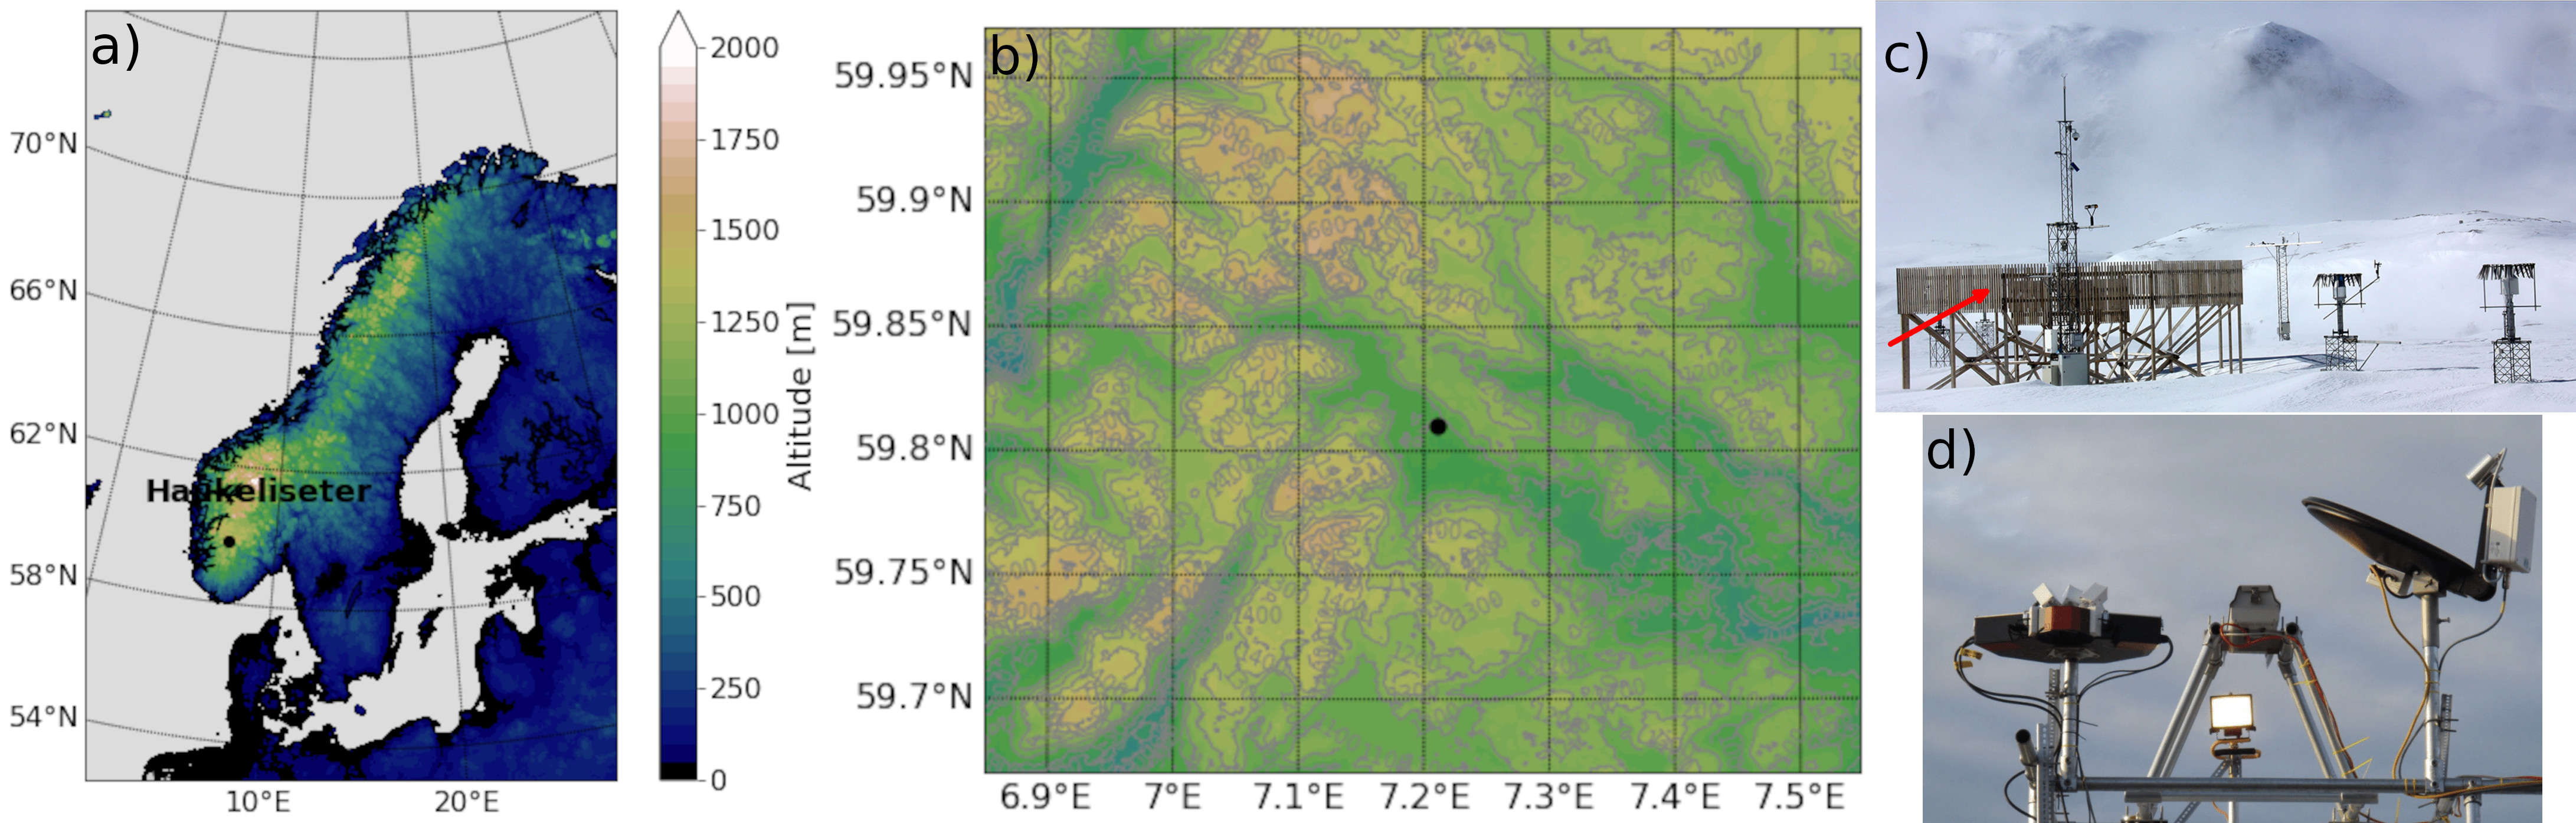
\includegraphics[width=19pc,angle=0]{fig1.jpg}\\
    \caption{a) Representation of the topography in MEPS and the MEPS model domain. HTS is located in the mountainous region in Southern Norway. The contours and shading present the elevation of the 2.5x2.5\,km grid cells. b) Topographic map around HTS. From the DTM 10 terrain model of \protect\citet{geonorge_dtm_2018}. HTS surrounded by 500\,m higher mountains to the west and more open to the south-east.
}
    \label{fig:norway_map}
\end{figure}

\begin{figure}[t]
    \noindent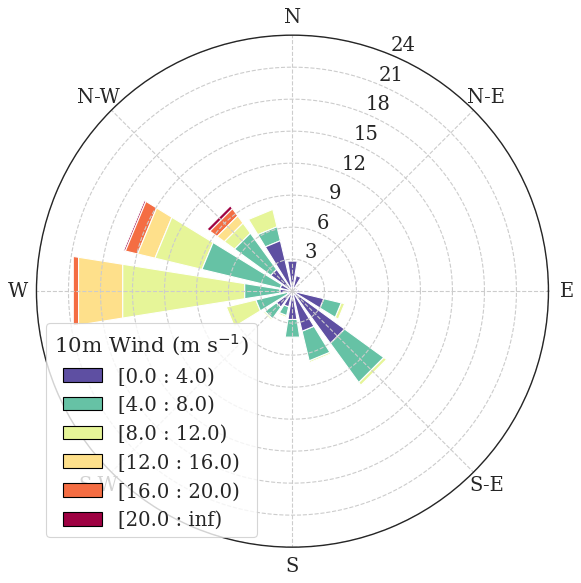
\includegraphics[width=19pc,angle=0]{fig2.png}\\
    \caption{Windrose of the 10-m wind during snowfall events when 24h accumulation $\geq$ 25\,mm\,d$^{-1}$ and 2-m temperature \textless 2\,$^{\circ}$C measured at HTS, during winter 2016-2017. Colors indicate the 10-m wind speed categories used in this study. 
}
    \label{fig:windrose}
\end{figure}

\begin{figure}[t]
    \noindent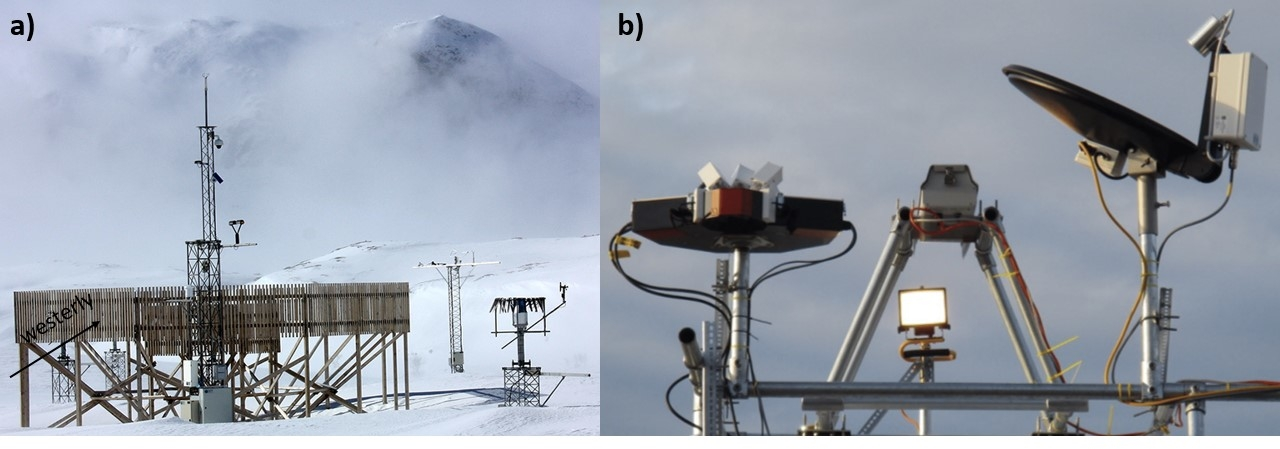
\includegraphics[width=19pc,angle=0]{fig3.jpg}\\
    \caption{a) DFAR, unprotected precipitation gauges and meteorological mast at HTS. The arrow indicates the westerly wind direction. The figure is adapted from \protect\citet{wolff_derivation_2015}. b) Additional instruments installed during HiLaMS during winter 2016-2017: Muli-Angular Snowflake Camera (MASC, left), Precipitation Imaging Package (PIP, middle), Micro Rain Radar (MRR, right).
}
    \label{fig:instruments}
\end{figure}

\begin{figure}[t]
    \noindent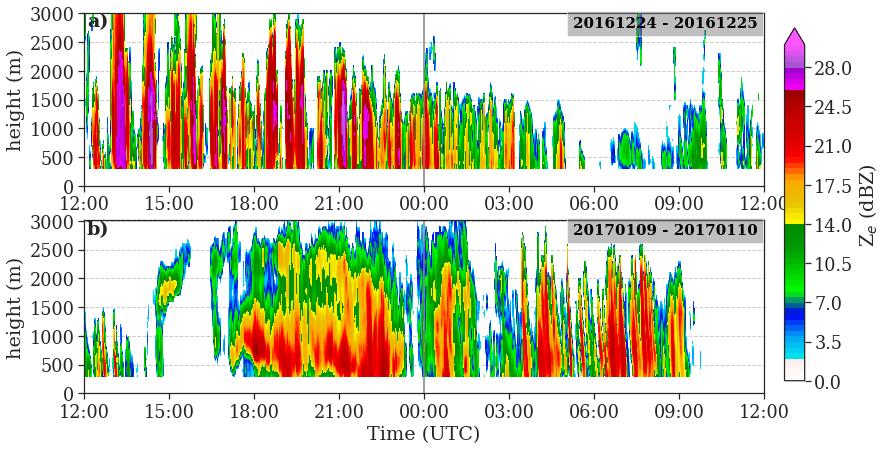
\includegraphics[width=19pc,angle=0]{fig4.png}\\
    \caption{Examples of MRR reflectivity during the two typical snowfall regimes. The time series for a westerly snowfall regime case during high wind speed on Dec 24-25 2016 (a). The westerly snowfall regime was associated with interchanging patterns of high and low reflectivities during snowfall. b) example during an easterly snowfall regime with low wind speeds and light precipitation of convective nature, on Jan 09-10 2017.
    }
    \label{fig:MRR_refl}
\end{figure}


\begin{figure}
    \noindent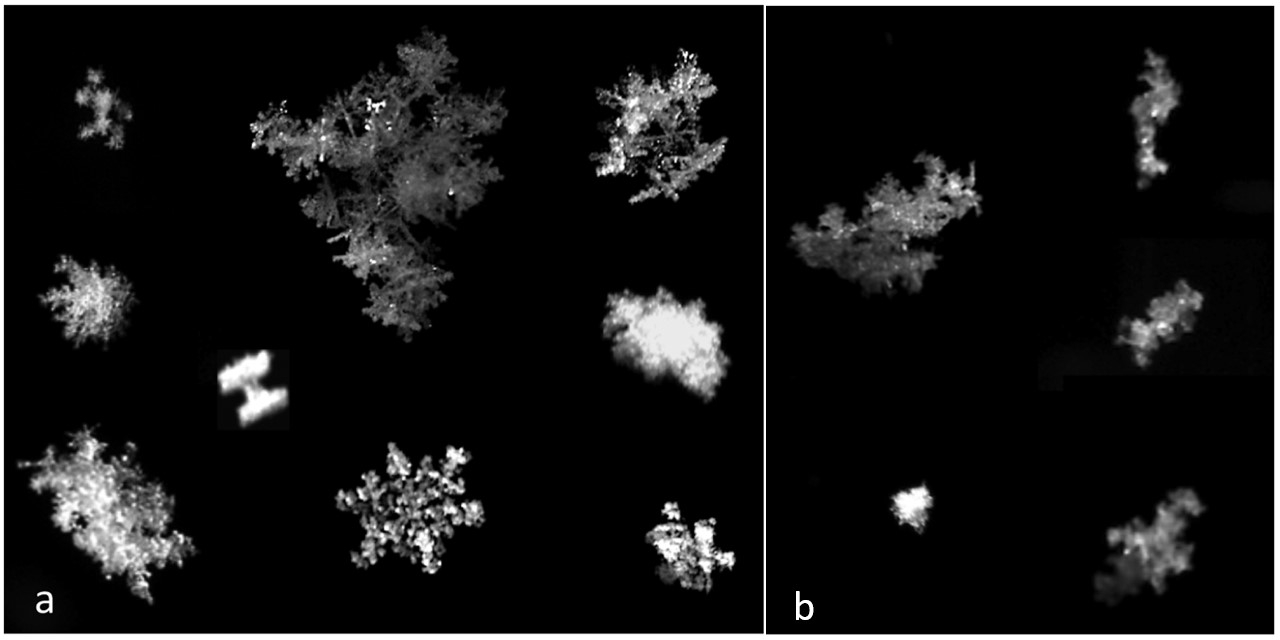
\includegraphics[width=19pc,angle=0]{fig5.jpg}\\
    \caption{a) Typical snowflake habits observed during events classified in the easterly snowfall regime. b) Examples of large precipitating crystals observed during the westerly snowfall regime. This figure is adapted from \protect\citet{schirle_estimation_2019}.
    }
    \label{fig:snowflakes}
\end{figure}

\begin{figure}
    \noindent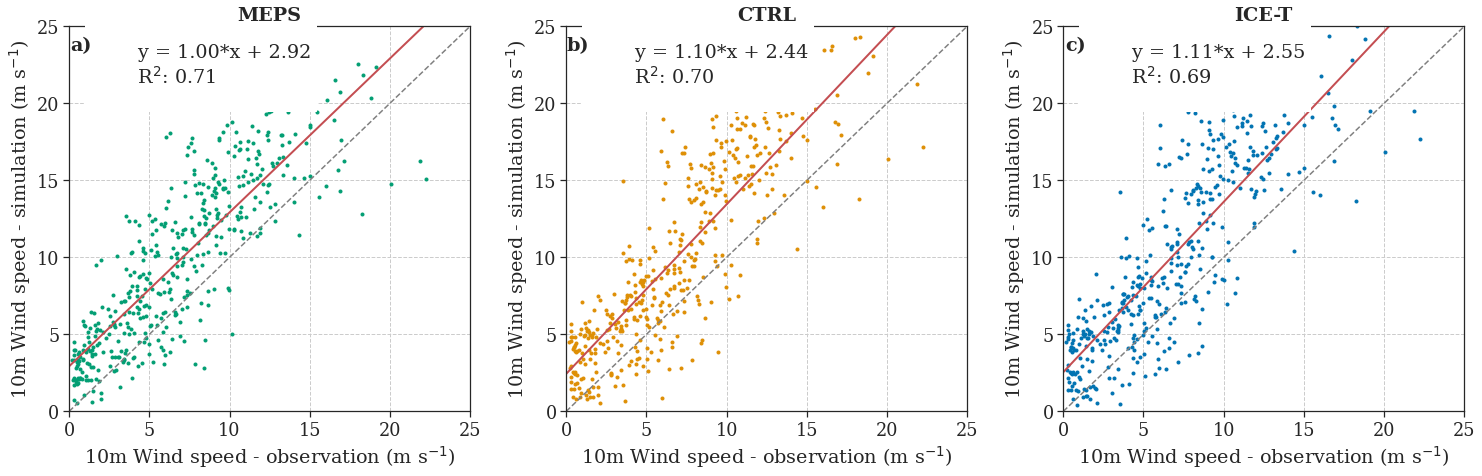
\includegraphics[width=19pc,angle=0]{fig6.png}\\
    \caption{Known 10-m wind bias \citep{frogner_convection-permitting_2019} was reduced according to the correlation equation between 10-m wind speeds observed at the DFAR and MEPS, CTRL, and ICE-T in a, b, and c, respectively. The red line indicates the linear correlation between DFAR and OESR.
    }
    \label{fig:WS_correlation}
\end{figure}


\begin{figure}
    \noindent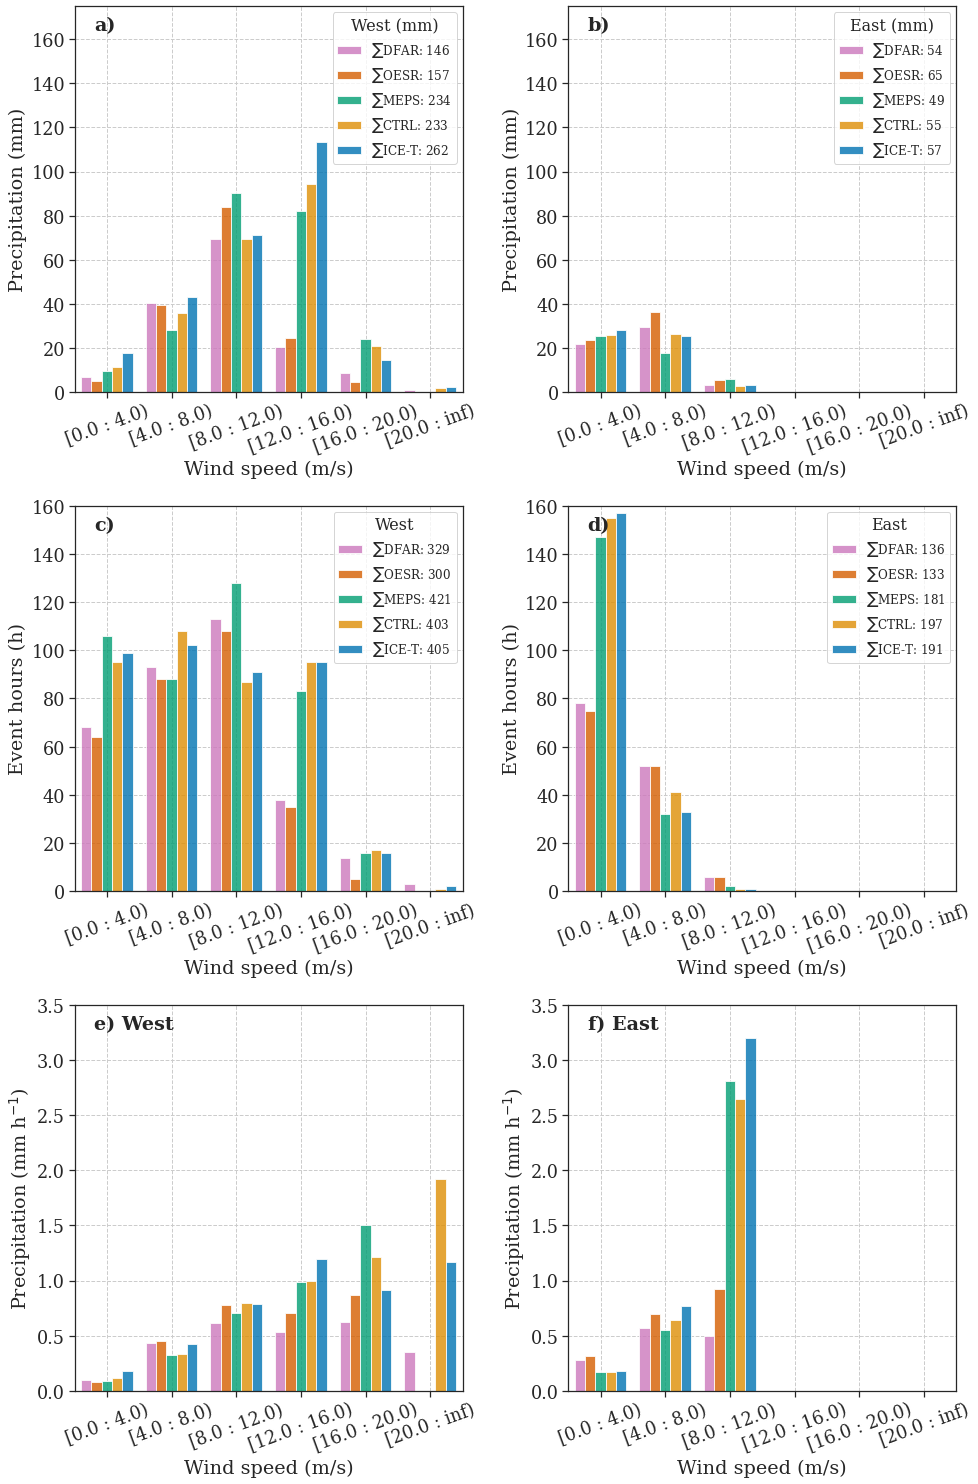
\includegraphics[width=19pc,angle=0]{fig7.png}\\
    \caption{Surface snowfall accumulation for DFAR observations, OESR, MEPS, CTRL, and ICE-T separated into westerly (a) and easterly (b) snowfall regimes for 27 precipitation days during winter 2016-2017. The sum of total precipitation accumulation in each snowfall regime is presented in the figure label in a and b. The separation into wind speed regimes is done for the corrected simulated wind according to the correlation equation in Fig. \ref{fig:WS_correlation} for MEPS, CTRL, and ICE-T. c and d show the event hours observed at the DFAR and OESR as well as the simulated precipitation hours in the NWPs. The total sum of the precipitation hours is presented in the figure label for the 27 precipitation days. Further, the snowfall accumulation is divided by the event hours in e) and f) for westerly and easterly, respectively.
    }
    \label{fig:sfc_WS_WD}
\end{figure}
    


\begin{figure}
    \noindent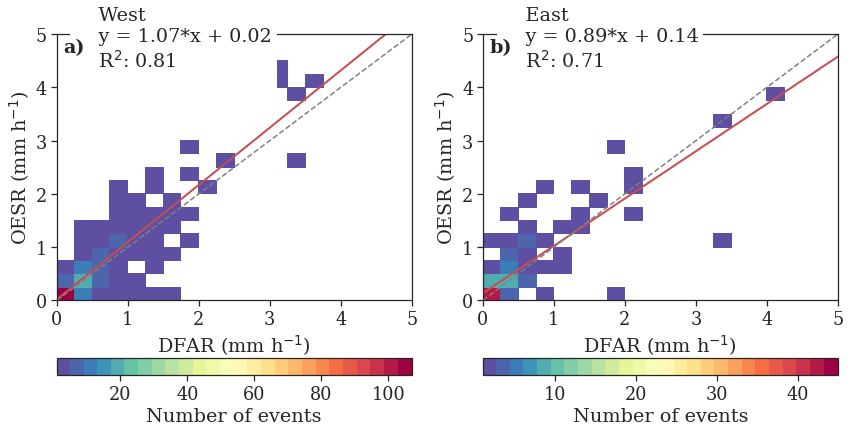
\includegraphics[width=19pc,angle=0]{fig8.png}\\
    \caption{Surface snowfall validation of OESR of the hourly snowfall accumulation, with DFAR observations on the x-axis and OESR estimates on the y-axis. The hourly accumulated snowfall amount is separated into westerly snowfall regime in a, and easterly snowfall regime in b. The red line indicates the linear correlation between the DFAR and the OESR surface snowfall accumulation. During westerly snowfall 121 events were counted at the 0.1\,mm\,h$^{-1}$ bin, while during easterly only 45 events were counted at the 0.1\,mm\,h$^{-1}$ bin.
}
    \label{fig:sfc_oesr}
\end{figure}




\begin{figure}
    \noindent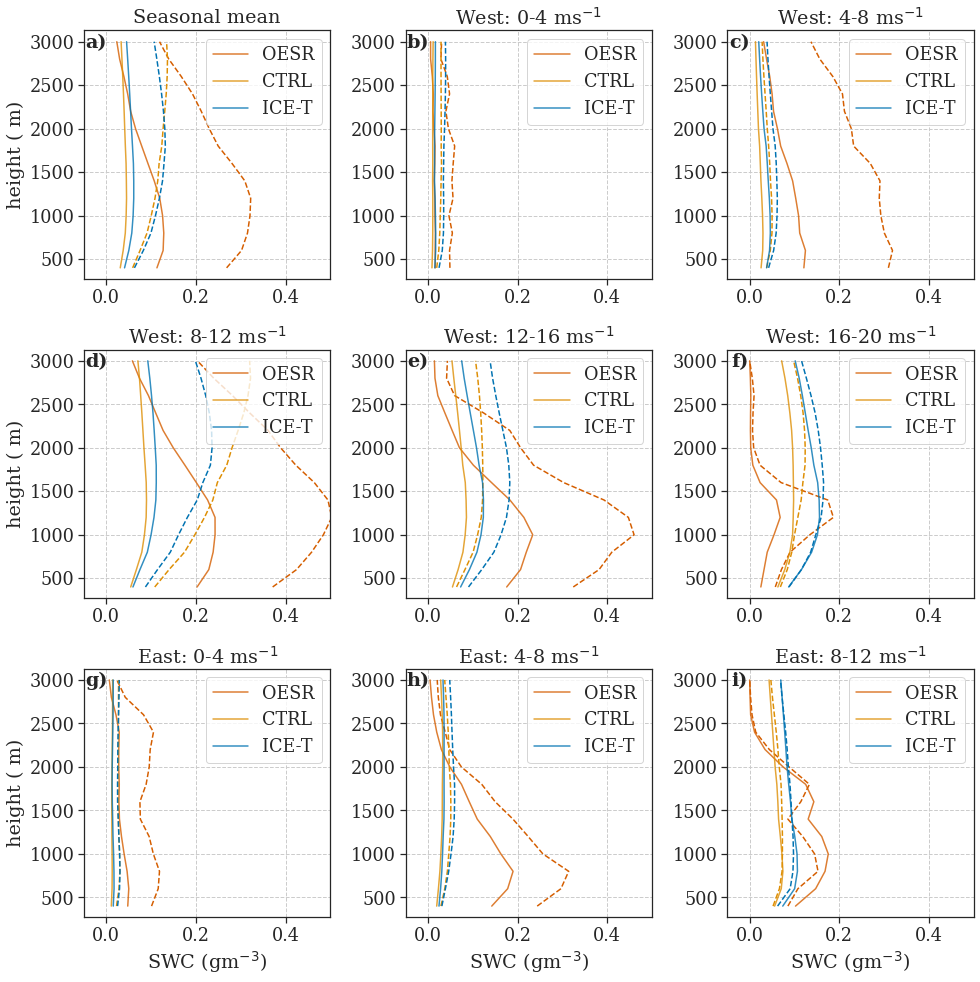
\includegraphics[width=19pc,angle=0]{fig9.png}\\
    \caption{Mean (solid) and standard deviation (dashed) of instantaneous SWC separated into west (a-f), east (g-i) snowfall regimes for days fulfilling the analysis requirements during winter 2016-2017. The SWC is sorted into snowfall regimes with the adjusted wind speed correction from the correlation equation in Fig. \ref{fig:WS_correlation}b and c for CTRL and ICE-T, respectively.
}
    \label{fig:vert_swc}
\end{figure}

\begin{figure}
    \noindent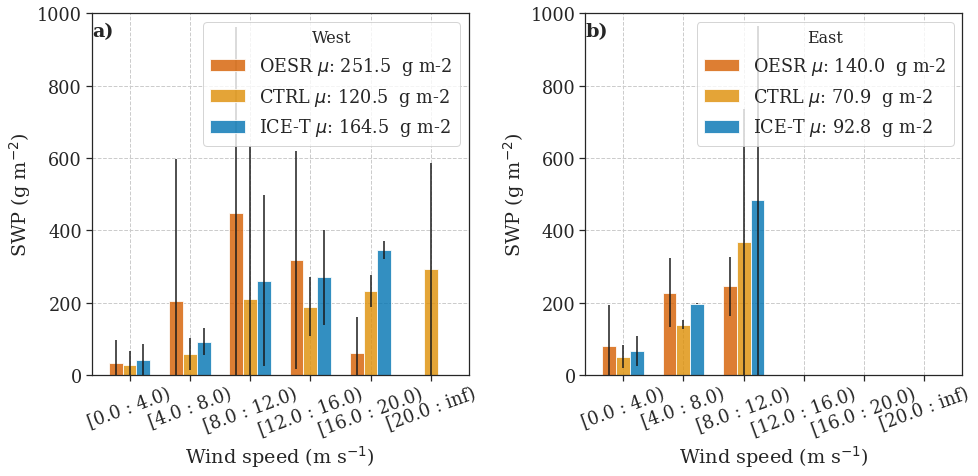
\includegraphics[width=19pc,angle=0]{fig10.png}\\
    \caption{Seasonal mean of instantaneous SWP for OESR, CTRL, and ICE-T forecasts separated into westerly and easterly snowfall regimes in a and b, respectively for 27 precipitation days during winter 2016-2017. The separation into wind speed is done with the corrected wind speed bias from Fig. \ref{fig:WS_correlation}b and c for CTRL and ICE-T, respectively. The black line indicates the standard deviation ($\pm \sigma$) in each snowfall wind regime. The mean and standard deviation in each wind speed bin is calculated individually hence the result is dependent on the event hours. The figure labels show the total mean of SWP for over all wind speed and all precipitation event hours. %mean SWP per hour
}
    \label{fig:swp_WS_WD}
\end{figure}
%
\end{document}